Back-propagation updates neural network weights $\rightarrow$ example
\visible<2->{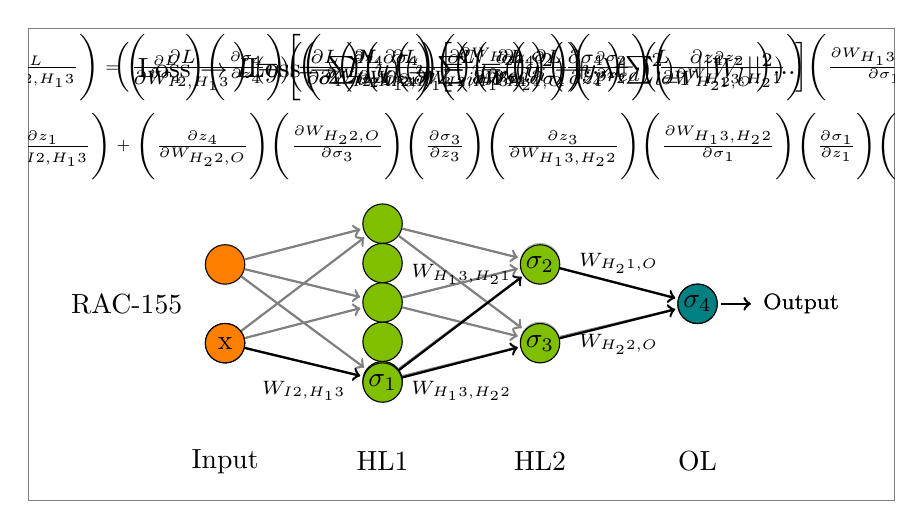
\begin{tikzpicture}[shorten >=1pt,draw=black, x=1cm, y=1 cm,  node distance=0cm]
	\draw[draw=gray, use as bounding box](-2.5,0) rectangle (8.5,6);
	\clip (-2.5,-0) rectangle (8.5,6);
	\def\layersep{2cm}
	\visible<7>{\node [] (ll) at (3,5.5) {Loss $\rightarrow L(y)=\sum_{i=1}^{N}((y_i-y_{pred})^2)$ };}
	\visible<8>{\node [] (ll) at (3,5.5) {Loss $\rightarrow L(y)=\sum_{i=1}^{N}((y_i-y_{pred})^2)+\lambda(\sum_{l=1}^{L}||W_l||^2)$ };}
	\visible<9>{\node [] (ll) at (3,5.5) {$\Big(\frac{\partial L}{\partial W_{I2,H_{1}3}}\Big)$};}
	\visible<10>{\node [] (ll) at (3,5.5) {$\Big(\frac{\partial L}{\partial W_{I2,H_{1}3}}\Big)=\Big(\frac{\partial L}{\partial \sigma_4}\Big)$};}
	\visible<11>{\node [] (ll) at (3,5.5) {$\Big(\frac{\partial L}{\partial W_{I2,H_{1}3}}\Big)=\Big(\frac{\partial L}{\partial \sigma_4}\Big)\Big(\frac{\partial \sigma_4}{\partial z_4}\Big)$};}
	\visible<12>{\node [] (ll) at (3,5.5) {$\Big(\frac{\partial L}{\partial W_{I2,H_{1}3}}\Big)=\Big(\frac{\partial L}{\partial \sigma_4}\Big)\Big(\frac{\partial \sigma_4}{\partial z_4}\Big)\Big[\Big(\frac{\partial z_4}{\partial W_{H_{2}1,O}}\Big)...+\Big(\frac{\partial z_4}{\partial W_{H_{2}2,O}}\Big)...\Big]$};}	
	\visible<13>{\node [] (ll) at (3,5.5) {\tiny$\Big(\frac{\partial L}{\partial W_{I2,H_{1}3}}\Big)=\Big(\frac{\partial L}{\partial \sigma_4}\Big)\Big(\frac{\partial \sigma_4}{\partial z_4}\Big)\Big[\Big(\frac{\partial z_4}{\partial W_{H_{2}1,O}}\Big)\Big(\frac{\partial W_{H_{2}1,O}}{\partial \sigma_2}\Big)\Big(\frac{\partial \sigma_2}{\partial z_2}\Big)\Big(\frac{\partial z_2}{\partial  W_{H_{1}3,H_{2}1}}\Big)\Big(\frac{\partial W_{H_{1}3,H_{2}1}}{\partial \sigma_1}\Big)$};}	
	\visible<13>{\node [] (ll) at (3,4.5) {\tiny$\Big(\frac{\partial \sigma_1}{\partial z_1}\Big)\Big(\frac{\partial z_1}{\partial W_{I{2},H_{1}3}}\Big)+\Big(\frac{\partial z_4}{\partial W_{H_{2}2,O}}\Big)\Big(\frac{\partial W_{H_{2}2,O}}{\partial \sigma_3}\Big)\Big(\frac{\partial \sigma_3}{\partial z_3}\Big)\Big(\frac{\partial z_3}{\partial  W_{H_{1}3,H_{2}2}}\Big)\Big(\frac{\partial W_{H_{1}3,H_{2}2}}{\partial \sigma_1}\Big)\Big(\frac{\partial \sigma_1}{\partial z_1}\Big)\Big(\frac{\partial z_1}{\partial W_{I{2},H_{1}3}}\Big)\Big]$};}
	%\visible<13>{\node [] (ll) at (3, 3.5){\tiny$\Big(\frac{\partial \sigma_1}{\partial z_1}\Big)\Big(\frac{\partial z_1}{\partial W_{I{2},H_{1}3}}\Big)$}}
    \tikzstyle{every pin edge}=[<-,shorten <=1pt,thick]
    \tikzstyle{neuron}=[circle,fill=black!25,minimum size=0.5cm ,inner sep=0pt, color=black, draw]
    \tikzstyle{input neuron}=[neuron, fill=green!50!blue!50];
    \tikzstyle{output neuron}=[neuron, fill=green!50!blue];
    \tikzstyle{hidden neuron}=[neuron, fill=green!50!orange];
    \tikzstyle{annot} = [text width=2em, text centered]
	\begin{scope}[x=1cm,y=1cm]
    % Draw the input layer nodes
    \foreach \name / \y in {2,3}{
        \visible<1>{\node[input neuron,fill=orange!100 ] (I-\name) at (0,\y) {$ $};}
	\visible<2->{\node[input neuron,fill=orange!100,opacity=0.25 ] (I-\name) at (0,\y) {$ $};}}
	 % Draw the hidden layer nodes
	 \visible<1>{\foreach \name / \y in {1,2,3}{
		 \path[yshift=0.5] node[hidden neuron] (H-\name) at (\layersep,\y+0.5) {\small $ $};}}
	\visible<1>{\foreach \name / \y in {2,3}{
		\path[yshift=0.5] node[hidden neuron] (H2-\name) at (\layersep,\y) {\small $ $};}}
		 %\path[yshift=0.5] node[hidden neuron] (H2-\name) at (2*\layersep,\y+0.5) {\small $ $};}}
		%%\path[yshift=0.5] node[hidden neuron] (H3-\name) at (3*\layersep,\y+0.5) {\small $ $};}
%		}
		
	  \visible<2->{\foreach \name / \y in {1,2,3}{
		 \path[yshift=0.5] node[hidden neuron, opacity = 0.25] (H-\name) at (\layersep,\y+0.5) {\small $ $};}}
	\visible<2->{\foreach \name / \y in {2,3}{
		 \path[yshift=0.5] node[hidden neuron, opacity = 0.25] (H2-\name) at (2*\layersep,\y) {\small $ $};}}
	 % Draw the output layer node
	 \visible<1>{\node[output neuron,pin={[pin edge={->}]right:\footnotesize Output}] at (3*\layersep,2.5) (O) {$ $};}
	\visible<2->{\node[output neuron, opacity=0.25,pin={[pin edge={->}]right:\footnotesize Output}] at (3*\layersep,2.5) (O) {$ $};}

	 \foreach \dest in {2,3}     
		 \foreach \source in {1,2,3}
		 {
			 \visible<1>{\path[thick,->,gray] (H-\source) edge node[font=\scriptsize] {} (H2-\dest) ;}\
			\visible<2->{\path[thin,->,gray] (H-\source) edge node[font=\scriptsize] {} (H2-\dest) ;}
%			 \path[thick,->,gray] (H2-\source) edge node[font=\scriptsize] {} (H3-\dest) ;
		}
 %        \foreach \dest in {2,4,6,8}

	 \end{scope}	             
    \foreach \source in {2,3}{
           \visible<1>{\path[thick,->,gray] (H2-\source) edge node[font=\scriptsize] {} (O) ;}
	\visible<2->{\path[thin,->,gray] (H2-\source) edge node[font=\scriptsize] {} (O) ;}}
    \foreach \source in {2,3}
		\foreach \dest in {1,2,3}  {   
        	\visible<1>{\path[thick,->,gray] (I-\source) edge node[font=\scriptsize] {} (H-\dest) ;}
	\visible<2->{\path[thin,->,gray] (I-\source) edge node[font=\scriptsize] {} (H-\dest) ;}}

%% call out node 1
%\node[circle, black,thick,minimum width = 2.7cm,minimum height = 2.7cm,path picture={\node at (path picture bounding box.center){\includegraphics[width=3cm]{representations/images/pisc_trans}}; }] (Xp) at (-1.24,5) {};
%\node[] (ll) at (3*\layersep,5) {$\Delta E_{H-L}$};

\visible<3->{\node[input neuron,fill=orange!100,opacity=1 ] (I-2) at (0,2) {x};}
\visible<3->{\node [] (ll) at (0,0.5) {Input};}
\visible<4->{\path[thick,->,black] (I-2) edge node[font=\scriptsize, midway,below=3pt,black] {{$W_{I2,H_{1}3}$}} (H-1) ;}
\visible<4->{\node[hidden neuron,opacity=1 ] (H-1) at (\layersep,1.5) {$\sigma_{1}$};}
\visible<4->{\node [] (ll) at (\layersep,0.5) {HL1};}
\visible<5->{\path[thick,->,black] (H-1) edge node[font=\scriptsize, midway, above=10pt,black] {$W_{H_{1}3,H_{2}1}$} (H2-3) ;}
\visible<5->{\path[thick,->,black] (H-1) edge node[font=\scriptsize, midway, below=3pt,black] {$W_{H_{1}3,H_{2}2}$} (H2-2) ;}
\visible<5->{\node[hidden neuron,opacity=1 ] (H2-2) at (2*\layersep,3) {$\sigma_{2}$};}
\visible<5->{\node[hidden neuron,opacity=1 ] (H2-2) at (2*\layersep,2) {$\sigma_{3}$};}
\visible<5->{\node [] (ll) at (2*\layersep,0.5) {HL2};}
\visible<6->{\path[thick,->,black, midway, below,black] (H2-2) edge node[font=\scriptsize] {$W_{H_{2}2,O}$} (O) ;}
\visible<6->{\path[thick,->,black, midway, above,black] (H2-3) edge node[font=\scriptsize] {$W_{H_{2}1,O}$} (O) ;}
\visible<6->{\node[output neuron,opacity=1] (O) at (3*\layersep,2.5) {$\sigma_4$};}
\visible<6->{\node [] (ll) at (3*\layersep,0.5) {OL};}
%\node [circle, fill=red, minimum size = 2cm] (mynode) at (3,3) {};
%\visible<2-3,5->{\node [circle, fill=blue, minimum size = 1cm,opacity=0.5] (mynode) at (3,3) {};}
%\only<2->{\node[circle, fill=green, minimum size = 2cm, below of = mynode] (mynode2) {};}
%\only<2->{\path[draw,very thick,black,->]  (mynode)--(mynode2);}
%    % Annotate the layers
	\node [] (ll) at (-1.25,2.5) {RAC-155};
\end{tikzpicture}}
